\RequirePackage[OT1]{fontenc} 
\documentclass[journal]{IEEEtran}

% *** CITATION PACKAGES ***
\usepackage[style=ieee]{biblatex} 
\bibliography{sources.bib}    %your file created using JabRef

% *** MATH PACKAGES ***
\usepackage{amsmath,amssymb}

% Table Packages
\usepackage{booktabs}
\usepackage{tabularx}

% *** PDF, URL AND HYPERLINK PACKAGES ***
% \usepackage{url}
\usepackage{hyperref, xcolor}
\hypersetup{
    colorlinks=true,
    linkcolor=blue,
    citecolor=blue,
    filecolor=blue,      
    urlcolor=blue,
    }

\urlstyle{same}

% correct bad hyphenation here
\hyphenation{op-tical net-works semi-conduc-tor}
\usepackage{graphicx}  %needed to include png, eps figures
\graphicspath{{./images/}}
\usepackage{float}  % used to fix location of images i.e.\begin{figure}[H]

%Mathcha
\usepackage{physics}
\usepackage{amsmath}
\usepackage{tikz}
\usepackage{mathdots}
\usepackage{yhmath}
\usepackage{cancel}
\usepackage{color}
\usepackage{siunitx}
\usepackage{array}
\usepackage{multirow}
\usepackage{amssymb}
\usepackage{gensymb}
\usepackage{tabularx}
\usepackage{extarrows}
\usepackage{booktabs}
\usetikzlibrary{fadings}
\usetikzlibrary{patterns}
\usetikzlibrary{shadows.blur}
\usetikzlibrary{shapes}
\usepackage{bigfoot} % to allow verbatim in footnote
\usepackage{listings}
\usepackage[final,numbered,framed]{matlab-prettifier}
\usepackage[T1]{fontenc} 
\begin{document}

\newcommand{\eqdef}{\mathrel{:\mathop=}}

%

% paper title

\title{The Impact of Quantum Computing on RSA}
%\\ \small{Title of the session (you can be creative highlighting your findings)}}

% author names 
% author names 
\author{Stephen Campbell \\
    \emph{sac170630@utdallas.edu} \\
    PHYS3330 --- Numerical Methods in Physics and Computational Techniques
}

% The report headers
\markboth{PHYS3330 Numerical Methods \today}%do not delete next lines
{PHYS3330 Numerical Methods \today}

% make the title area
\maketitle

% As a general rule, do not put math, special symbols or citations
% in the abstract or keywords.
\begin{abstract}
    The RSA cryptosystem plays an ever important role in the security of the modern
    internet. Simultaneously, the threat of quantum computing inches closer to
    obliterating this system entirely. This project is an effort to explore and
    understand the algorithms and methodology behind RSA and the quantum
    computing ``lightsaber'' the cripples its integrity. Through a hands on
    approach, the algorithms involved in the topics explored are written up as
    python scripts that allow such methods to be easily understood, analyzed,
    and validated.
\end{abstract}

\section{Introduction}
\IEEEPARstart{P}{op} science media portrays quantum computing as the next
greatest computing revolution. Inspired by a talk given by Helwer
\cite{Helwer2018}, this project explores the motivation, applications, and
technical methods in the grandiose topic of quantum computation. Specifically,
motivation behind prime factorization is cultivated through the exposition of
the RSA cryptosystem. Then, the current classical methods are shown and Shor's
algorithm \cite{Shor1997}, the quantum alternative to these methods, is analyzed
and implemented. In an effort to have a hands on experience with the technical
topics discussed, many algorithms apart of these topics were reimplemented in
python from scratch. The scripts apart of this effort and the \LaTeX  source of this report are
hosted on a github repo
\href{https://github.com/Stephen-Campbell-UTD/NM_Project_Quantum_Computing}{here}.



\section{RSA}

Public key cryptosystems are the basis of secure communication on the internet.
The Rivest-Shamir-Adleman (RSA) \cite{Rivest1978} public key cryptosystem is prominently used on
the modern internet. In fact, it is currently being used in the browser I am
writing this in! Understanding how RSA functions and how quantum computing
"breaks" it provides tantamount evidence of the application of the computational
power leveraged by quantum computers.

\subsection{Purpose}

In a public key cryptosystem, a participant generates a pair of keys : the
public key and the private key. The public key is openly distributed and allows
anyone to encrypt information. Ideally, this encrypted information can only be
decrypted with the private key. This ideal cryptosystem does not exist. The goal
of RSA and of modern public key cryptosystems, is to create a practical
methodology to generate a public and private key such that it is effectively
impossible to decrypt encrypted data without the private key.

\subsection{Mechanics}

There are 3 major computational components of the RSA cryptosystem: key
generation, encryption, and decryption. As a note on general terminology, an
encrypted message is referred to as a ciphertext.  The setup of RSA is that a
public key, in the form a tuple of numbers \((e, n)\), is generated and
distributed. The private key is also a kept as tuple of numbers \((d,n)\);
however this key is not distributed .  A concise explanation of the
cryptosystem follows.

\subsubsection{Encryption}

The encryption step of RSA is one fairly straightforward calculation. The
ciphertext \(c\) is generated from the message \(m\) by the below equation.

\begin{align*}
    c & \eqdef m^{e}\bmod n
\end{align*}

\subsubsection{Decryption}

The decryption step of RSA is also a straightforward calculation. The
ciphertext is decrypted by the below equation.

\begin{align*}
                            & 0\leqslant m< n         \\
    \left( m^{e}\right)^{d} & \equiv m\quad (\bmod n)
\end{align*}

\subsubsection{Key generation}

The steps of encryption and decryption feel magical, yet rely on very unique
properties that exist between the modulus, the encryption key, and the
decryption key. These special properties will be developed shortly. First, there
are important theorems that are utilized.

\begin{align*}
                  & \text{Euler's Totient Function}                                                       \\
    n             & =p_{1}^{k_{1}} p_{2}^{k_{2}} \dotsc p_{r}^{k_{r}}                                     \\
    \varphi ( n)  & =p_{1}^{k_{1} -1}( p_{1} -1) p_{2}^{k_{2}}( p_{2} -1) \dotsc p_{r}^{k_{r}}( p_{r} -1) \\
                  & \text{Euler's Theorem}                                                                \\
    \gcd( n,a) =1 & \Longrightarrow a^{\varphi ( n)} \equiv 1\ \bmod n
\end{align*}

The major idea is shown below.

\begin{align*}
    m                    & \eqdef \text{Message}                                              \\
                         & \text{Choose}                                                      \\
    n                    & :0\leqslant m< n                                                   \\
                         & \text{Then}                                                        \\
    m                    & =m\left( m^{\varphi ( n)}\right)\bmod n\ \text{Assume m,n coprime} \\
    m                    & =m\left( m^{\varphi ( n)}\right)^{h}\bmod n                        \\
    m                    & =m^{h\varphi ( n) +1} \ \bmod n                                    \\
    m^{h\varphi ( n) +1} & =m^{ed}\bmod n                                                     \\
    h\varphi ( n) +1     & =ed,\ h\in \mathbb{Z}                                              \\
    ed                   & =1\bmod \varphi ( n)                                               \\
                         & \text{Choose}                                                      \\
    e                    & :0< e< \varphi ( n) ,\ \gcd\left( e,\varphi ( n)\right) =1\        \\
                         & \text{Find Modular Inverse of } e
\end{align*}

After the encryption key \(e\) is found, the decryption \(d\) key can be easily
determined by computing the modular inverse.

\subsection{What makes this hard to crack?}

As seen from the key generation step, the decryption key can be easily recovered
from the encryption key and the Euler totient function \(\varphi(n)\) of the modulus. The
modulus and the encryption key are both distributed as the public key. The
Euler totient function is extremely easily to calculate for a prime number, it
is simply \(p-1\); however, for a composite the totient function requires the
complete prime factorization of the composite. This provides the connection
between cracking RSA and prime factorization.   Furthermore, to make factoring
problem harder and the cryptosystem more secure, 2 extremely large prime numbers
are chosen. These numbers have roughly half the bits of the modulus. So for a
2048 bit key, the modern standard, these prime numbers are 1024 bits or on the order of \(10^{308}\).

\subsection{A Curious Aside}

As seen from the key generation step, the decryption key can be easily recovered
from the encryption key and the Euler totient function of the modulus. The
modulus and the encryption key are both distributed as the public key . The
Euler totient function is extremely easily to calculate for a prime number, it
is simply p-1;however, however for a composite the totient function requires the
complete prime factorization of the composite . This provides the connection
between cracking RSA and prime factorization.   Furthermore, to make factoring
problem harder and the cryptosystem more secure, 2 extremely large prime numbers
are chosen. These numbers have roughly half the bits of the modulus. So for a
2048 bit key, these prime numbers are 1024 bits or on the order of \(10^{308}\).

\subsection{Classical Cracking}

One method of cracking RSA would be to factor the publicly distributed modulus.
With the prime factorization of modulus in hand, one could calculate the Euler
totient of the modulus, take the inverse of the encryption key \(\bmod\)the totient of the
modulus and recover the decryption key. Thus, the major problem lies in
factoring the modulus. The goto algorithms for factoring large integers are the
general number field sieve and the quadratic sieve. The general number field
sieve considered slightly better for integers \(> 10^{100}\), and  has an asymptotic running
time of
\[\exp\left(\left(\sqrt[3]{\frac{64}{9}} +o( 1)\right)(\ln n)^{1/3}(\ln\ln n)^{2/3}\right) \]
What does this all mean? The state of the art \cite{Zimmermann2020} in classical factorization is when
a number compliant to RSA-250 (on the order of 10e250) was factored. The
calculation was performed on an array of Intel Xeon Gold 6130 CPUs and the
combined duration was roughly 2700 ``core'' years.

\section{Quantum Computing}
In an effort to achieve insights into applications of quantum computing, a hands
on approach to learning about the topic was taken. The Qiskit provided textbook and associated
labs of \url{https://qiskit.org/textbook/preface.html}
proved enormously helpful in shedding light on this topic in this project's
limited timeframe. Qiskit provides a python module for quantum circuit
construction and simulation. This python module was utilized to create a python
implementation of Shor's algorithm. Conveyed below are key takeaways from this
resource.
\subsection{Fundamentals}
\textbf{Definitions}
\begin{itemize}
    \item A qubit is any two state quantum mechanical system.
    \item A quantum gate is a unitary transformation on the state of a set of qubits.
    \item A quantum computer refers to a construction of connections between qubits and quantum gates.
\end{itemize}
Many quantum gates are useful in constructing high level circuits. These
include: Controlled Not, Toffoli, Pauli X, Y, Z, Hadamard, Controlled Phase, and
Fredkin. The action of these gates is easily seen when visualized on the Bloch
sphere. The Qiskit visualization library provides convenience methods that plot
the state of the qubits in a quantum circuit. An example is depicted below in
Fig.~\ref{fig:BlochSphere}.

\begin{figure}[H]
    \begin{center}
        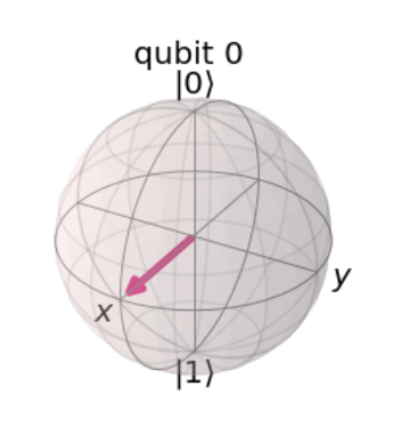
\includegraphics[width=0.35\textwidth]{BlochSphere.png}
        \caption{\label{fig:BlochSphere} A Qubit in the \(\ket{+}\) state represented on the Bloch Sphere}
    \end{center}
\end{figure}

\subsection{Building Blocks}
\subsubsection{Quantum Fourier Transform}

From a practical viewpoint, the quantum Fourier transform is a unitary
transformation that maps a set of qubits encoded in binary to a set of qubits
encoded in a "Fourier" basis. Essentially, this Fourier basis encodes the binary
number as a phase around the z axis. A phase of 0 points along the axis. An
example from the Qiskit website is shown below in Fig \ref{fig:FourierBasis}.


\begin{align*}
    \ket{q_{3} q_{2} q_{1} q_{0}} & =\ket{0101}                                                                                              \\
    \operatorname{QFT}\ket{0101}  & =\ket{q_{3} 'q_{2} 'q_{1} 'q_{0} '}                                                                      \\
    q_{0} '                       & \rightarrow \frac{1}{\sqrt{2}}\left(\ket{0} +\exp\left( 2\pi i\cdot \frac{5}{2^{4}}\right)\ket{1}\right) \\
    q_{1} '                       & \rightarrow \frac{1}{\sqrt{2}}\left(\ket{0} +\exp\left( 2\pi i\cdot \frac{5}{2^{3}}\right)\ket{1}\right) \\
    q_{2} '                       & \rightarrow \frac{1}{\sqrt{2}}\left(\ket{0} +\exp\left( 2\pi i\cdot \frac{5}{2^{2}}\right)\ket{1}\right) \\
    q_{3} '                       & \rightarrow \frac{1}{\sqrt{2}}\left(\ket{0} +\exp\left( 2\pi i\cdot \frac{5}{2^{1}}\right)\ket{1}\right)
\end{align*}

\begin{figure}[H]
    \begin{center}
        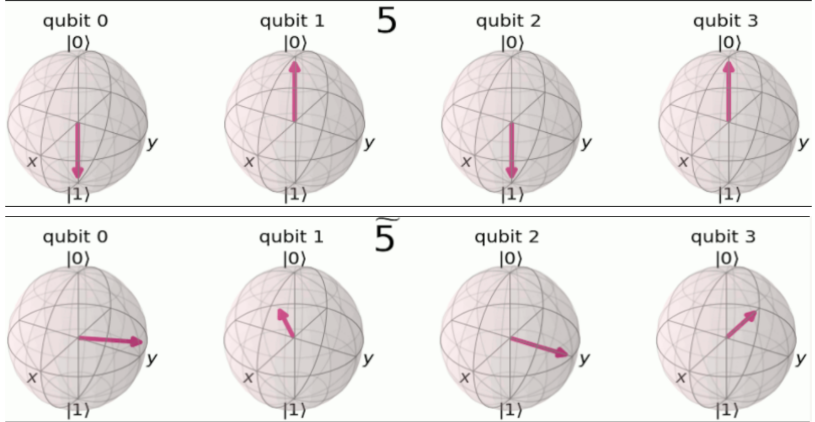
\includegraphics[width=0.35\textwidth]{FourierBasis.png}
        \caption{\label{fig:FourierBasis} The number 5 encoded in the binary basis and the Fourier basis }
    \end{center}
\end{figure}


Constructing the quantum Fourier transform circuit relies only on 2 gates: the Hadamard and
controlled phase gate. A 3 Bit QFT circuit is shown in Fig. \ref{fig:QFTCirc}.

\begin{figure}[H]
    \begin{center}
        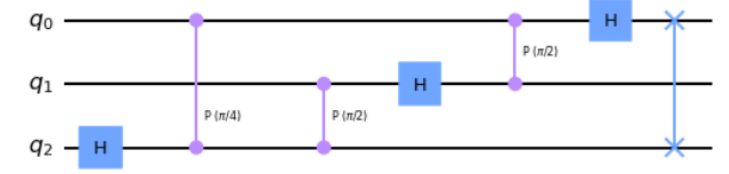
\includegraphics[width=0.35\textwidth]{QFTCirc.png}
        \caption{\label{fig:QFTCirc} 3 Bit QFT Circuit}
    \end{center}
\end{figure}

\subsubsection{Quantum Phase Estimation}

The purpose of a quantum phase estimation circuit is to approximate the
eigenvalue of a unitary operator's eigenstate. Given the eigenstate can be
prepared and the unitary operator can be applied, the circuit allows for
arbitrary precision approximation by increasing the number of approximating
qubits. As to be seen, the problem of integer factorization can be reduced to
estimating the phase of a unitary operator. In Shor's algorithm, in regards to
exactly how many qubits are required for integer factorization, Shor recommends
twice the number of qubits needed to represent the number we are trying to
factor.

\subsubsection{Quantum Modular Exponentiation}

As Shor notes in his praised paper, "The bottleneck in the quantum factoring
algorithm; i.e., the piece of the factoring algorithm that consumes the most
time and space, is modular exponentiation."\cite{Shor1997} Interestingly, the
modular exponentiation algorithm he presents is simply a quantum, and thus
reversible, version of a classical circuit. Implementing this modular
exponentiation circuit with Qiskit proved similar to be of the acclaimed
complexity. The design implemented was heavily inspired from Vedral's
exposition \cite{Vedral1996} on arithmetic operations on quantum computers. The
procedure of the design was the following:

\emph{Carry and Sum Blocks}

All addition and subtraction operation begin by adding the left operand's bit,
the right operand's bit, and a potential "carry" bit from the previous
operation. In quantum circuits, these blocks can be realized with toffoli and
cnot gates.

\begin{figure}[H]
    \begin{center}
        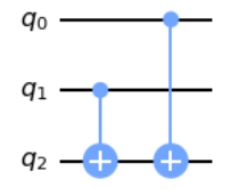
\includegraphics[width=0.35\textwidth]{Sum.png}
        \caption{\label{fig:Sum} A Classic Sum Block Implemented with Quantum Gates}
    \end{center}
\end{figure}

\begin{figure}[H]
    \begin{center}
        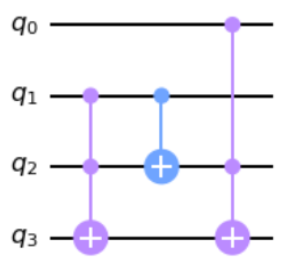
\includegraphics[width=0.35\textwidth]{Carry.png}
        \caption{\label{fig:Carry} A Classic Carry Block Implemented with Quantum Gates}
    \end{center}
\end{figure}

\emph{N Qubit Adder}

A n bit adder can be constructed with a cascade of sum and carry blocks. Because
the circuit must be reversible, the circuit requires the use of "ancilla" bits
where intermediate values are computed and ``uncomputed''.

\begin{figure}[H]
    \begin{center}
        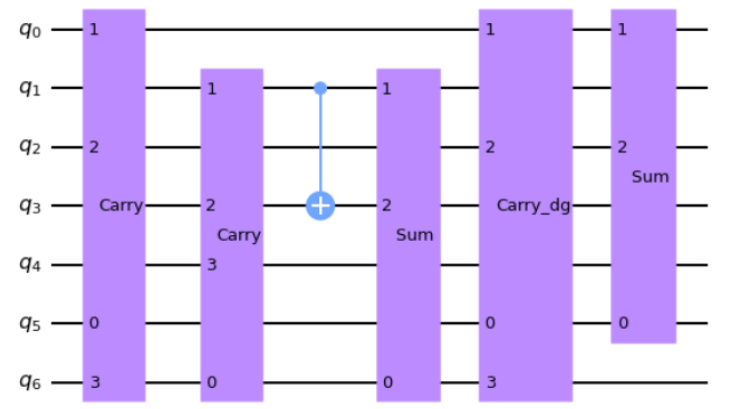
\includegraphics[width=0.35\textwidth]{Adder.png}
        \caption{\label{fig:Adder} A 2 Bit Adder Block Implemented with Carry and Sum Blocks }
    \end{center}
\end{figure}

\emph{N Qubit Modular Adder}

The adder's inverse, noted in the example as adder dg, has the effect of
subtracting the left operand from the right. This fact is utilized in the
modular adder.  The process of the modular adder circuit is as follows:

\begin{enumerate}
    \item The modulus is placed in qubits 7 and 8, the left operand is in qubits 0-1, the right operand in 2-4, 5-6 are ancilla, qubit 9  is also ancilla
    \item The left and right operand are added
    \item The modulus is then subtracted from that addition
    \item The sign bit is "copied" to the ancillary qubit 9 and the modulus is added back if necessary
    \item The value of the sign bit is uncomputed to make the gate reversible
\end{enumerate}

\begin{figure}[H]
    \begin{center}
        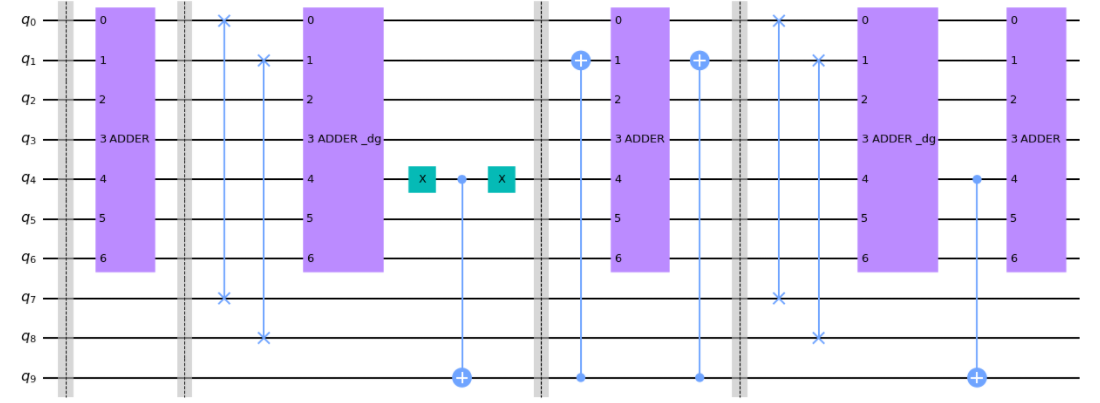
\includegraphics[width=0.35\textwidth]{ModAdder.png}
        \caption{\label{fig:ModAdder} A 2 Bit \(\bmod 2\) Adder Block Implemented with Adder Blocks }
    \end{center}
\end{figure}

\emph{Controlled N Qubit Modular Multiplier}

By "Classically Controlling" the position of the gates based on the one of the
multiplication's operands and utilizing the properties of modular
multiplication, the quantum controlled modular multiplication circuit can be
realized.

\begin{figure}[H]
    \begin{center}
        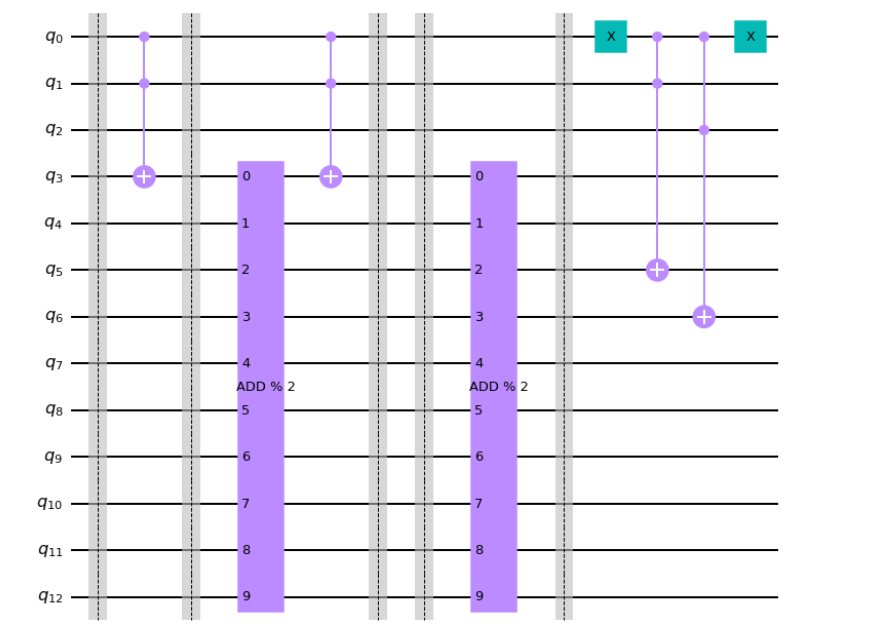
\includegraphics[width=0.35\textwidth]{CModMult.png}
        \caption{\label{fig:CModMult} A 2 Bit Mod 2 Multiply by 3 Controlled
            Modular Multiplier Block Implemented with Modular Adder Blocks }
    \end{center}
\end{figure}

\emph{Controlled N Qubit Modular Exponentiation}

The modular exponentiation circuit can be realized by cascading controlled
modular multiplications and uncomputing ancillas when necessary.

\subsection{Shor's Algorithm}
The goal of Shor's algorithm is to find the period, \(r\), of a number, \(b
\bmod n \). With \(r\), the number \(n\) can be factored. This is shown below.

\begin{align*}
    a^{r}                                            & \equiv 1\bmod n            \\
    a^{r} +1                                         & =nq,\ q\ \in \mathbb{Z}    \\
    \text{Restart if}                                & \ r\%2\ =1\                \\
    \text{Restart if}                                & \ a^{r} \equiv -1,1\bmod n \\
    \left( a^{r/2} +1\right)\left( a^{r/2} -1\right) & =nq,\ q\ \in \mathbb{Z}    \\
    \gcd\left( a^{r/2} -1,n\right)                   & =\text{Factor of } n
\end{align*}


Using a quantum computer, the period of a number \(\bmod n\) can be found by
using phase estimation on the unitary operator \(b\cdot x \bmod N\) on a state
\(\ket{x}\). The eigenstate chosen to find the period is simply \(\ket{1}\) .
The phase estimated will be some fraction whose denominator has a high
probability of being the period, \(r\), of a number, \(b \bmod n\).  On a quantum
computer, this algorithm shatters the classic asymptotic complexity for integer factorization:
\[
    O\left((\log n)^{2}(\log\log n)(\log\log\log n)\right)
\]
With this said, while traditional quantum computers do not currently pose a
threat via large integer factorization, what is exciting is that the asymptotic
complexity is polynomial rather than exponential. If quantum computers could
easily scale the size of the circuits and the number of qubits, this quantum
superiority would be on full display.

\section{Conclusion and Key Takeaways}

Through the exploration involved in the project, the abilities quantum circuits
provide have been shown to be of great importance. In a bittersweet manner,
Shor's algorithm has yet to see practical use. This is simply because the number
of ``ideal'' qubits required to crack RSA with Shor's algorithm is much more
than the state of the art. It is predicted that Shor's Algorithm will be viable
in the future and it is simply a matter of time. While seemingly concerning,
there have been discussions regarding so-called ``Post-Quantum'' cryptography.
These are systems intended to be immune to the threats posed by the quantum
computing revolution.

This project has led to the discovery of many impactful resources and
technologies, especially in \href{https://qiskit.org/}{Qiskit}. Alongside these discoveries, some key technical
takeaways are

\begin{itemize}
    \item There is an enormous amount of engaging resources about quantum computing and its simulation
    \item Cryptography provides great motivation for topics in number theory
    \item Quantum Computing topics usually have large overlap with ideas from classical digital logic systems
\end{itemize}

% \bibliographystyle{IEEEtran}
% \bibliography{example_bib}
\printbibliography

% \appendices
% \section{Pre-Lab}
% \section{Extra Photos}

\end{document}